%% Based on a TeXnicCenter-Template by Gyorgy SZEIDL.
%%%%%%%%%%%%%%%%%%%%%%%%%%%%%%%%%%%%%%%%%%%%%%%%%%%%%%%%%%%%%
%
%------------------------------------------------------------
%
\documentclass[a4paper,12pt,reqno]{article}
%----------------------------------------------------------
\usepackage{amsfonts}
\usepackage{graphicx}
\usepackage{geometry}
\usepackage{color}
\usepackage{amssymb,amsmath}
\usepackage{polski}
\usepackage[T1]{fontenc}
\usepackage[utf8]{inputenc}
\usepackage{caption}
\geometry{margin=1.1in}
\usepackage{wrapfig}
\usepackage{lipsum}  
\usepackage{listings}
\usepackage[toc,page]{appendix}
\usepackage{url}

\definecolor{codegreen}{rgb}{0.5, 0.09, 0.09}
\definecolor{codegray}{rgb}{0.5,0.5,0.5}
\definecolor{codepurple}{rgb}{0.58,0,0.82}
\definecolor{backcolour}{rgb}{0.94,0.94,0.94}
\definecolor{gray}{rgb}{0,0.6,0}

\lstdefinestyle{mystyle}{
    backgroundcolor=\color{backcolour},  
    commentstyle=\color{codegreen},
    keywordstyle=\color{blue},
    numberstyle=\tiny\color{codegray},
    stringstyle=\color{codepurple},
	basicstyle=\footnotesize\fontfamily{cmtt}\selectfont,
    breakatwhitespace=false,         
    breaklines=true,
    captionpos=b,
	language=C++,
    keepspaces=true,                 
    numbers=left,                    
    numbersep=5pt,                  
    showspaces=false,                
    showstringspaces=false,
    showtabs=false,                  
    tabsize=2
}
 
\lstset{style=mystyle}
\lstset{literate=%
    *{0}{{{\color{gray}0}}}1
    {1}{{{\color{gray}1}}}1
    {2}{{{\color{gray}2}}}1
    {3}{{{\color{gray}3}}}1
    {4}{{{\color{gray}4}}}1
    {5}{{{\color{gray}5}}}1
    {6}{{{\color{gray}6}}}1
    {7}{{{\color{gray}7}}}1
    {8}{{{\color{gray}8}}}1
    {9}{{{\color{gray}9}}}1
}
%------------------------------------------------------------
\begin{document}

%\begin{figure}[h]
%	\centering
%		\includegraphics[width=0.40\textwidth]{logo.pdf}
%\end{figure}


\begin{center}

\thispagestyle{empty}

%UNIWERSYTET WROCŁAWSKI\\
\Large 
Uniwersytet Wrocławski\\
Wydział Fizyki i Astronomii\\
\vspace{0.8cm}
\vspace{1.8cm}

\Large Krzysztof Kukiz \\
\vspace{3.2cm}
\Large \textbf{INTELIGENTNE POWITANIE} \\
\vspace{1.5cm}
INTELLIGENT GREETING
\end{center}
\vspace{3.7cm}
\begin{flushright}
\large{ Praca inżynierska na kierunku \\Informatyka Stosowana i Systemy Pomiarowe \\}
\vspace{0.5cm}
\large{ Opiekun \\ dr hab. Maciej Matyka, prof. UWr}
\end{flushright}
\vspace{2.2cm}

\begin{center}
\large Wrocław, \today
\end{center}

\newpage

\tableofcontents

\newpage

\begin{flushleft}
\Large \textbf{Streszczenie}
\end{flushleft}
\vspace{1cm}
Niniejsza praca przedstawia projekt systemu inteligentnego rozpoznawania osób oraz podejmowania przez system wcześniej zdefiniowanych działań, w zależności od rozpoznanej osoby. W przypadku braku rozpoznania osoby, system poda także odpowiedni komunikat głosowy oraz wizualny.
\begin{itemize}
  \item List entries start with the \verb|\item| command.
  \item Individual entries are indicated with a black dot, a so-called bullet.
  \item The text in the entries may be of any length.
\end{itemize}

\newpage
\begin{flushleft}
\Large \textbf{Abstract}
\end{flushleft}
\vspace{1cm}
Po angielsku

\newpage

\section{Wstęp}
abcd efgh
\subsection{Wprowadzenie}
\subsection{Cel i zakres pracy}
\subsection{Struktura pracy}

\newpage
\section{Wymagania stawiane projektowi}

\newpage
\section{Oczekiwane funkcjonalności projektu}

\newpage
\section{Warstwa sprzętowa}
\subsection{Kamera jako element wejściowy}
\subsection{Płyta Raspberry Pi}
\subsection{Głośnik jako element wyjściowy}

\newpage
\section{Warstwa programistyczna}
\subsection{Python jako język programowania}
\subsection{Algorytm}
\subsection{Kod}

\newpage
\section{Warstwa produktowa}
\subsection{Technologia druku 3D}
\subsection{Projekt obudowy}
\subsection{Wykonanie obudowy}

\newpage
\section{Realizacja projektu}
\subsection{Napotkane problemy}
\subsection{Możliwości rozbudowy}

\newpage
\section{Wnioski}

\newpage

\bibliographystyle{plain}
\bibliography{praca_dyplomowa_krzysztof_kukiz}


\newpage

\begin{equation} 
\rho\left(\frac{\partial\vec v}{\partial t}+(\vec v\cdot\nabla)\vec v\right) =\rho\vec f - \nabla p + \mu\triangle\vec v, \label{rownanie}
\end{equation} 

\begin{figure}[!ht]%
\centering
\includegraphics[scale=0.85]{logo.eps}
\caption{Podpis rysunku, który jest obrazem wektorowym (EPS). \label{logotyp}}
\qquad
\end{figure}   

\begin{figure}[!ht]%
\centering
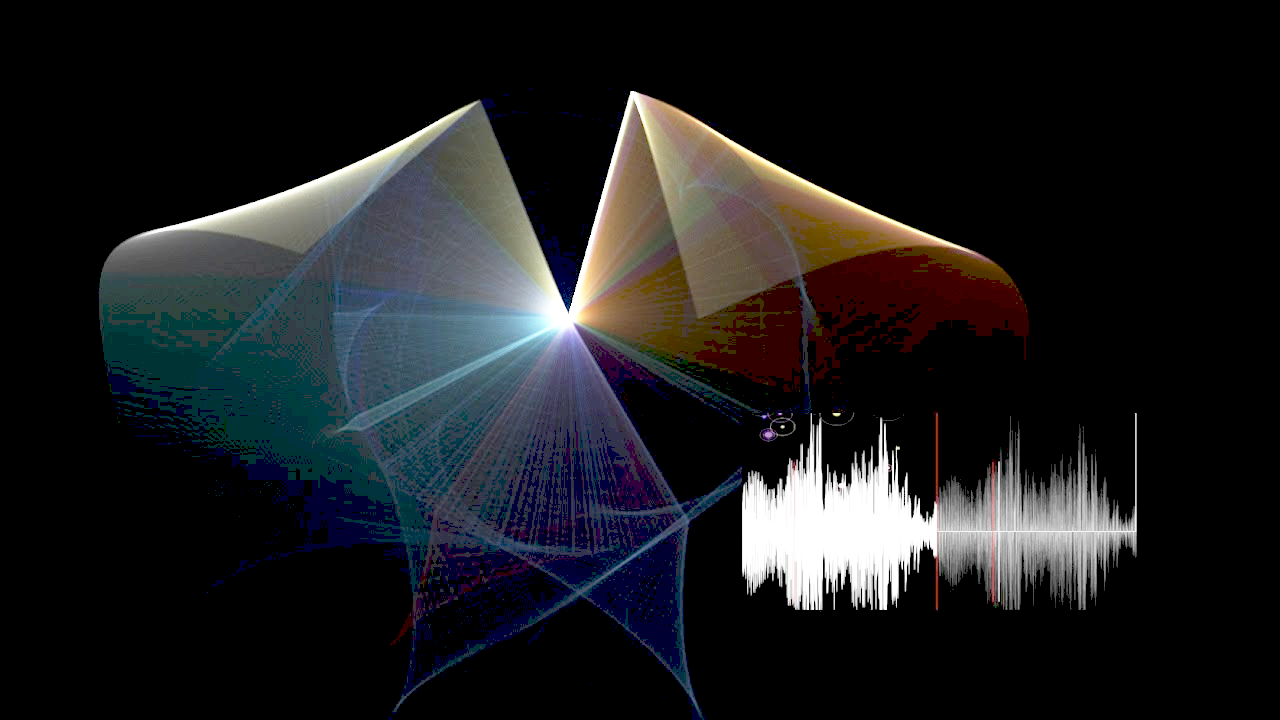
\includegraphics[width=0.8\columnwidth]{pendulums.png}
\caption{To jest rysunek drugi, kilkadziesiąt wahadeł podwójnych z syntezą dźwięku.\label{wahadla}}%
%
\qquad
\end{figure} 

\end{document}




